%Copyright (c)  2005-2010 EDF-EADS-PHIMECA.
%  Permission is granted to copy, distribute and/or modify this document
%  under the terms of the GNU Free Documentation License, Version 1.2
%  or any later version published by the Free Software Foundation;
%  with no Invariant Sections, no Front-Cover Texts, and no Back-Cover
%  Texts.  A copy of the license is included in the section entitled "GNU
%  Free Documentation License".
\renewcommand{\etapemethodo}{C}
\renewcommand{\nomfichier}{docref_C322_LHS}
\renewcommand{\titrefiche}{Latin Hypercube Simulation}

\Header

\MathematicalDescription{

\underline{\textbf{Goal}}\\
Let us note $\mathcal D_f = \{\ux \in \mathbb R^{n_X} \space | \space  g(\ux,\underline{d}) \leq 0\}$.
The goal is to estimate the following probability:
\begin{eqnarray*}
P_f  &=& \int_{\mathcal D_f} f_{\uX}(\ux)d\ux\\
     &=& \int_{\mathbb R^{n_X}} \mathbf{1}_{\{g(\ux,\underline{d}) \leq 0 \}}f_{\uX}(\ux)d\ux\\
     &=& \Prob {\{\space g(\uX,\underline{d}) \leq 0 \}}
\end{eqnarray*}

\underline{\textbf{Principles}}\\

LHS or \space Latin Hypercube Sampling is a sampling method enabling to better cover the domain of variations of the input variables, thanks to a stratified sampling strategy. This method is applicable in the case of independent input variables.  The sampling procedure is based on dividing the range of each variable into several intervals of equal probability. The sampling is undertaken as follows:

\begin{itemize}
\item   \textbf{Step n�1}\ \ The range of each input variable is stratified into isoprobabilistic cells,
\item	\textbf{Step n�2}\ \ A cell is uniformly chosen among all the available cells,
\item \textbf{Step n�3}\ \ The random number is obtained by inverting the Cumulative Density Function locally in the chosen cell,
\item \textbf{Step n�4}\ \ All the cells having a common strate with the previous cell are put apart from the list of available cells.
\end{itemize}

The estimator of the probability of failure with LHS is given by:
$$
\hat{P}_{f,LHS}^N = \frac{1}{N}\sum_{i=1}^N \mathbf{1}_{\{g(\uX^i,\underline{d}) \leq 0 \}}
$$
where the sample of $ \{ \uX^i,i=1 \hdots N \}$ is obtained as described previously.\\
One can show that:
$$
\Var{\hat{P}_{f,LHS}^N} \leq \frac{N}{N-1} . \Var{	\hat{P}_{f,MC}^N}
$$
where:
\begin{itemize}
\item	$\Var {\hat{P}_{f,LHS}^N}$ is the variance of the estimator of the probability of exceeding a threshold computed by the LHS technique,
\item	$\Var {\hat{P}_{f,MC}^N}$ is the variance of the estimator of the probability of exceeding a threshold computed by a crude Monte Carlo method.
\end{itemize}


\underline{\textbf{Confidence Interval}}\\
With the notations,
\begin{eqnarray*}
\mu_N &=& \frac{1}{N}\sum_{i=1}^N \mathbf{1}_{\{g(\underline{x}_i),\underline{d}) \leq 0 \}}\\
\sigma_N^2 &=& \frac{1}{N}\sum_{i=1}^N (\mathbf{1}_{\{g(\underline{x}^i),\underline{d}) \leq 0 \}} - \mu_N)^2
\end{eqnarray*}

the asymptotic confidence interval of order $1-\alpha$ associated to the estimator $P_{f,LHS}^N$ is 
$$
[ \mu_N - \frac{q_{1-\alpha / 2} . \sigma_N}{\sqrt{N}} \space ; \space \mu_N + \frac{q_{1-\alpha / 2} . \sigma_N}{\sqrt{N}} ]
$$
where $q_{1-\alpha /2}$ is the $1-\alpha / 2$ quantile from the reduced standard gaussian law $\mathcal N(0,1)$.

It gives an unbiased estimate for $P_f$ (reminding that all input variables must be independent).

}
{
% Autres notations et appellations
This method is derived from a more general method called 'Stratified Sampling'.
}

\Methodology{
This method is part of the step C of the global methodology. It requires the specification of the joined probability density function of the input variables and the definition of the threshold. The PDF must have an independent copula.
}
{

\begin{itemize}
\item	This method \textit{a priori} enables a better exploration of the domain of variations of the input variables. No general rule can guarantee a better efficiency of the LHS sampling than the classical Monte Carlo sampling. Nevertheless, one can show that the LHS strategy leads to a variance reduction if the model is motoneous over each variable.
\item Be careful, this method is valid only if the input random variables are independent!
\item Moreover, for reliability problems, when the failure probability is low, the tails of the distributions usually contain the most influent domains in terms of reliability. 
\item A fruitful link towards the global approach can be established with the files
\end{itemize}	


\otref{docref_C321_MonteCarloStd}{Monte Carlo Method to evaluate a probability to exceed a threshold}, \\
\otref{docref_C322_TI}{Importance Sampling to evaluate a probability to exceed a threshold} coming from the methodology. 

}

\Example{
To illustrate this method, we consider the sampling strategy of an input vector of dimension 2. Both components follow a uniform law $\mathcal U(0,1)$.
The figure compares the population of 30 points obtained by a Latin Hypercube Sampling and by a Monte Carlo Sampling.

\begin{center}
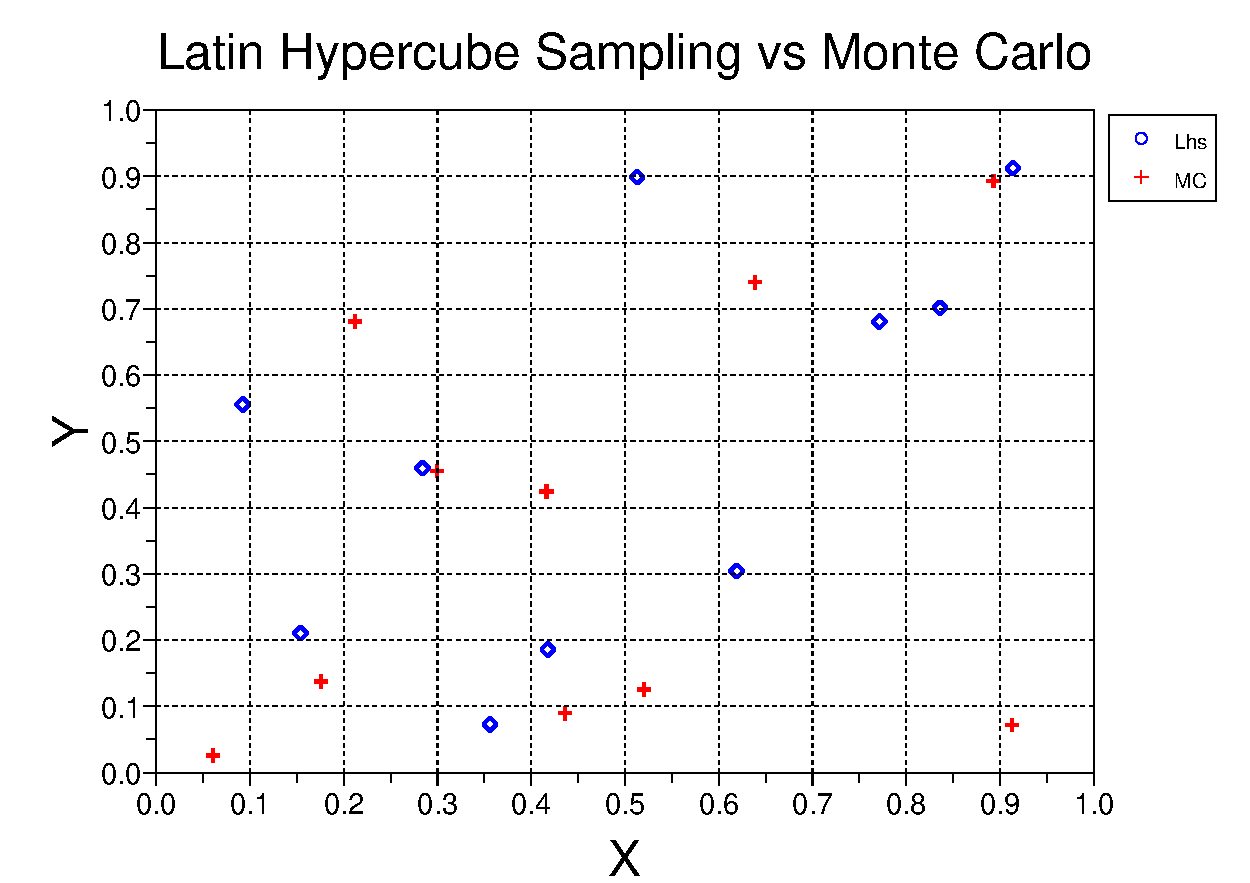
\includegraphics[width=0.80\textwidth]{LHS_vs_MC.pdf}
\end{center}

With the LHS sampling strategy, each row and each column is filled by a blue square whereas some row and column do not contain any red cross.

}
